% Domain, Problem, Literature review, Solution, methodology and What this report does
\section{Introduction}

\subsection{Domain and problem}
In this project, the key domain is natural language processing (NLP), which focuses on extracting information, such as emotions or opinions, from the given content. The reviews of movie classification is a classic problem where sentiment, including positive and negative, is predicted based on the context of reviews, its applications are verity including renewcommand systems and business intelligence. The primary challenge is to capture the nuances and semantic relationships in the content accurately particularly when dealing with the complex language. 

\subsection{Literature review}
A research \cite{pang2008opinion} introduces machine learning (ML) techniques to classify the review depend on its sentiment, which achieves high accuracy in prediction of audience opinions. It is a practical application for this kind of project to understanding the viewers' preferences and improve the film industry's decision making. 

Pang et al. (2022) pioneered using ML for movie review sentiment classification \cite{pang2002thumbs}, and more recent works demonstrate that ensemble methods like Random Forests, outperform simpler models such as Naive Bayes, or Logistic Regression in many real-world settings \cite{breiman2001random,go2009twitter}. Moreover, datasets like the Standford IMDB dataset \cite{maas2011learning} have become benchmarks for evaluating models. Random Forest is chosen as one candidate due to its robustness and effectiveness in high-dimensional textual content classification \cite{kowsari2019text}. 

Long-Short-Term Memory (LSTM) has also shown a significant advantages in textual content sentiment analysis. For instance, Johnson and Zhang (2016) introduced an efficiently LSTM framework which is using a general "region embedding plus pooling" paradigm \cite{johnson2016supervised}. They feed one-hot vectors into LSTM units instead of the word embedding layer. In this architecture, they built a one-hot bidirectional LSTM with pooling (oh-2LSTMp), which achieved a test error rate by 8.14\%, and in the supervised setting by 6.66\%. Sachan et al. (2019) developed a bidirectional LSTM model, which trained with supervised and semi-supervised losses, the model achieved 4.32\% error rate on IMDB dataset \cite{sachan2019revisiting}.

Deep learning (DL) has revolutionized ability to solve NLP problems by enabling models to learn complex patterns from large datasets. It surpasses traditional ML approaches in the sentiment analysis tasks. The DL models, such as recurrent neural networks (RNNs) and convolutional neural networks (CNNs), extract features from the content automatically. However, these models often struggling with capturing long dependencies, which limits its performance in the tasks. 

Devlin et al. (2018) introduce Bidirectional Encoder Representations from Transformers (BERT) to handle this tasks with significant advancement. BERT leverages a bidirectional transformer architecture, which allows it to capture the context from preceding and following words. It combines with pre-trained on vast corpora and next-sentence prediction, which enables BERT to generate rich representations \cite{Devlin2018}. In sentiment analysis, BERT excels by modeling complex relationships between words in textual content. For example, Sun et al. (2019) demonstrated BERT's advantage in sentiment analysis, it outperforms RNNs and CNNs, and achieves robust performance with limited labeled data \cite{Sun2019}. However, this methods also cause challenges such as computational complexity and resource demands.

\subsection{Dateset}
The IMDB dataset is widely used benchmark for sentiment classification. It contains 50,000 movie reviews collected from the Internet Movie Database (IMDB), and it is split into 25,000 positive and same number of negative reviews equally, which means that it is a balanced dataset. This feature ensures no class imbalance issues which influences the accuracy of the results. Each review is labeled as either positive by 1 or negative by 0, making it a binary classification task. This dataset is originally divided into training (50\%) and testing (50\%) sets. All selected methods are trained and evaluated on this dataset.

\begin{figure}[ht]
    \centering
    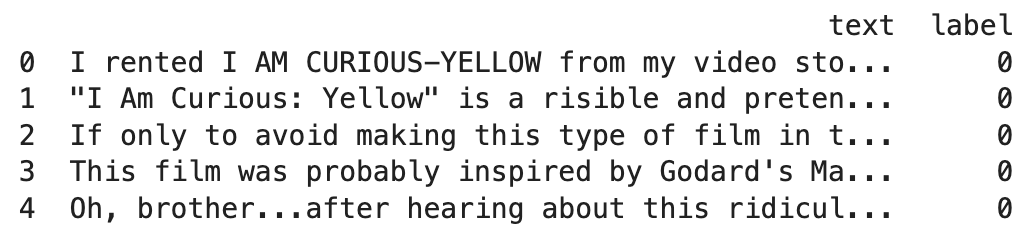
\includegraphics[width=0.8\textwidth]{pics/data_sample.png}
    \caption{Dataset samples}
\end{figure}

\subsection{Solution}
To address the sentiment classification task based on IMDB \cite{stanfordnlp2025imdb}, we propose three distinct machine learning models: Random Forest, LSTM networks and BERT. These models are selected to capture a long range of dependencies, from traditional methods to advanced deep learning techniques, which allows us to compare their effectiveness in this textual classification. Random Forest leverages tree-based learning, LSTM captures sequential dependencies in content, and BERT utilizes contextual embeddings to understand semantic representations. After evaluation, our goal is to identify the most effective approach for Sentiment classification on the selected dataset.

The methodology for this study involves the following steps:
\begin{enumerate}
    \item Data Preprocessing
    \item Model Implementation
    \item Training and Evaluation
    \item Comparison and Analysis
\end{enumerate}


\subsection{What this report does}
This report compares Random Forest, LSTM, and BERT in the sentiment classifying task. It details the implementation, training and evaluating for each model, then it provides insights into their strengths and weaknesses. It also demonstrates the processing steps, feature engineering techniques and fine tuning method. To compare and analyzing the results, the recommendations on the most suitable model are identified for sentiment classification, which contributes how traditional and deep learning approaches perform on textual content.